\section{Unity}
Glavno sučelje od unity-a se može vidjeti na slici \ref{fig:unitysucelje}. Raspored koji se može vidjeti je najoptimalniji za rad ukoliko programer ima samo jedan monitor. U slučaju da programer ima više monitora onda bi se mogao napraviti puno pregledniji raspored. 

\subsection{Inspektor}
Inspektor (\emph{eng. Inspector}) se koristi za provjeravanje pojedinih opcija komponenta igrajućih objekata (\emph{eng. GameObject}). Pomoću njega je moguće dodavati elemente i obavljati bilo koju operaciju, te vidjeti sve moguće stavke o objektu.

\begin{figure}[h]
	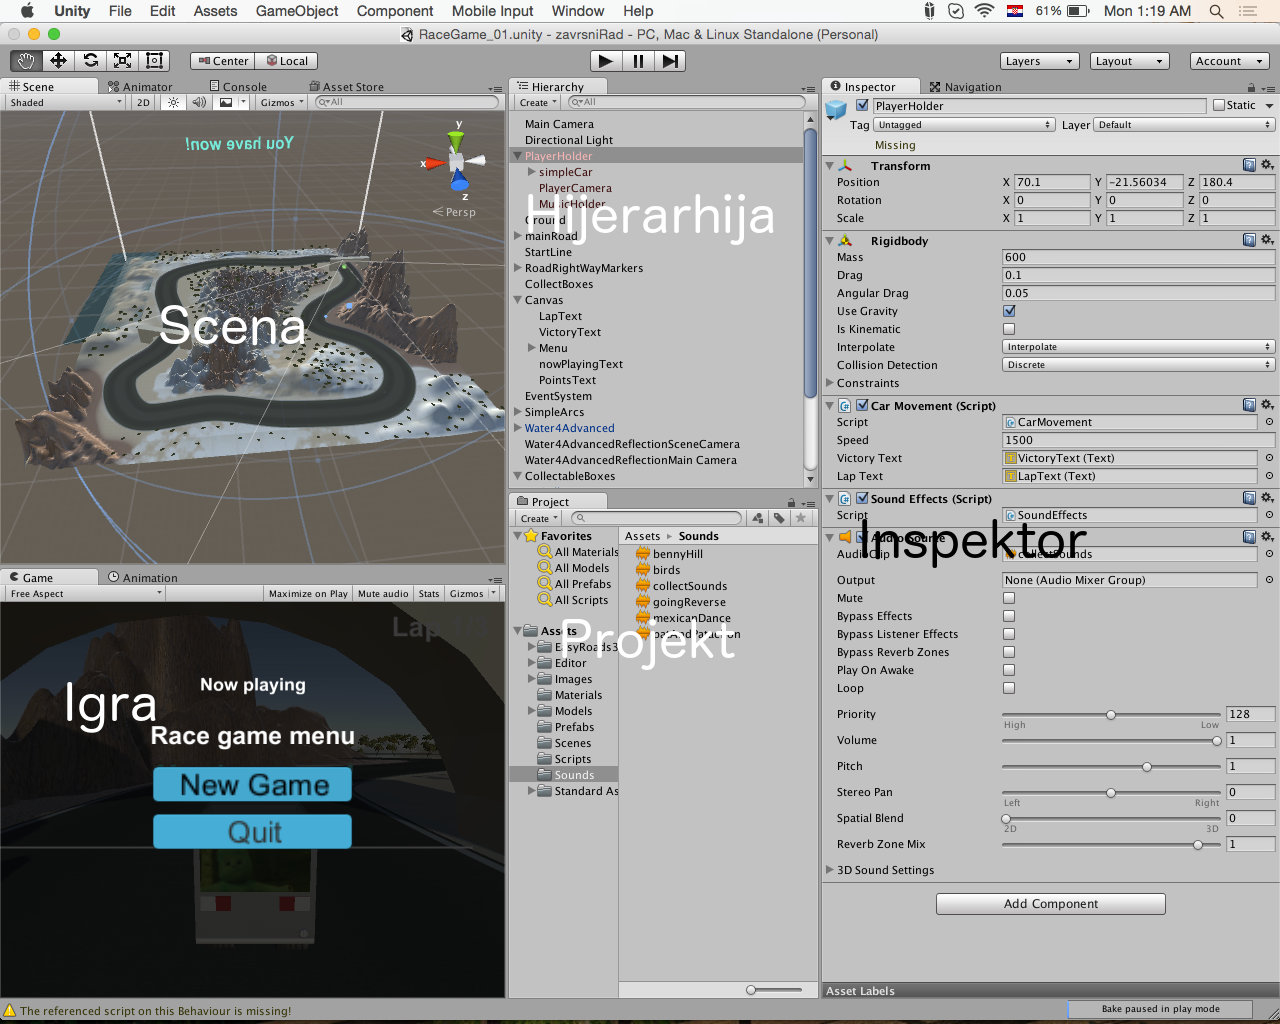
\includegraphics[width=12.5cm, height=10cm]{unitysucelje.png}
	\centering
	\caption{Unity sučelje}
	\label{fig:unitysucelje}
\end{figure}
\newpage

\subsection{Scena}
Scena (\emph{eng. Scene}) se koristi prilikom izrade igre kako bi se moglo iz neutralne pozicije gledati cijeli svijet. Sve preinake koje se rade u svijetu kao što su dodavanje objekata, određivanje položaja, dimenzija se obavljaju unutar ovog dijela. U gornjem desnom kutu se može vidjeti maleni objekt koji je crvene, zelene i plave boje. On programeru govori trenutnu orijentaciju u svijetu. Zelena boja je y, crvena je x, a plava z koordinata.

\subsection{Hijerarhija}
Hijerarhija (\emph{eng. Hierarchy}) je dio u kojem se nalaze svi igrajući objekti koji su napravljeni. Ovdje je moguće vidjeti odnos svih igrajućih objekata. Pod odnos se misli na roditelj, dijete, gdje jedan igrajući objekt može biti dijete drugog. Na ovaj način je moguće iz roditelja pristupati djeci i njihovim komponentama. Iako unity pruža mogućnost i obrnutog procesa, ovo ugnježđivanje omogućuje jednu odličnu funkcionalnost koja se koristi u igri. Ako je kamera dijete nekog objekta koji se pokreće sa nekom silom, tada kamera prati kretenje tog igrajućeg objekta i dobiva se iluzija kao u 3D igricama gdje se glavni junak gleda iz trećeg lica. 

\subsection{Projekt}
Projekt (\emph{eng. Project}) segment omogućava programeru da vidi sve datoteke koje su uključene u igru i njihovu hijerarhiju. Zbog praktičnosti se naprave direktoriji za skripte, zvukove, modele i ostale objekte koji će se ponavljati kroz igru, kako bi se što lakše mogli pronaći prilikom rada. Postoji ugrađeni pretraživač za još jednostavnije pronalaženje željenih datoteka, kao i različiti filteri.

\subsection{Igra}
Ovaj dio je ono što igrač vidi kada pokrene igru, a omogućava programeru da što zornije postavi parametre kako bi igra izgledala kako je on zamislio. Moguće je postaviti da prilikom pokretanja igre u unity-u se poveća slika na maksimum (\emph{eng. maxmizie on play}). Pokretanje igre je kao slušanje glazbe u bilo kojem alatu. Postoje igraj (\emph{eng. play}), pauziraj i pomak po slici.

\subsection{Konzola}
Konzola (\emph{eng. Console}) se koristi za provjeravanja koda unutar igre. Moguće je logove ispisivati za provjeru pojedinih varijabli tokom igranja i provjeravanja okidača da li uistinu rade. Bilo koja greška koja nije uzrokovana tijekom rada će prvo biti prikazana u konzoli crvenom bojom sa oznakom linije i imenom skripte u kojoj se dogodila greška.

\subsection{Trgovina}
Trgovina (\emph{eng. Asset store}) se koristi za kupnju ili nabavljanje gotovih modela preko interneta, koje je netko drugi već napravio. U slučaju ove igre, cesta je preuzeta sa trgovine jer sama izrada ceste bi bio preduogtrajan proces. Trgovina ima svoje filtere za pojedine kategorije igara i tipova objekata koji su potrebni.

\subsection{Igrajući objekti}
Svaki objekt koji se može vidjeti u unity-u je \textbf{igrajući objekt}. Kada se napravi bilo koj objekt on treba imati svoju poziciju unutar svijeta. Kako bi se mogla znati njegova pozicija koristimo komponente. Svaki objekt mora imati svoju transformaciju (\emph{eng. Transform}). U suštini igrajući objekti su samo kontenjeri koji sadrže komponente.

\subsection{Kamera}
Kamere se koriste za prikaz igre kako je programer zamislio. Koristeći više kamera moguće je napraviti različite efekte i animacije za igrača, te stvoriti jedinstveno iskustvo tijekom igranja igre. Kamere imaju dvije moguće projekcije (ortografijsku i perspektivnu). Ortografijska se koristi za 2D igrice ili ako nije bitna dubina u igricama. Najčešće su to neke platformske igre, puzzle ili slično. Perspektivna se koristi ako je želimo pokazati dubinu u igri. U igri se koristi ovaj oblik, te je postavljena kao dijete automobilskog igrajućeg objekta. Na ovaj način kamera slijedi automobil i dobiva se pravo iskustvo vožnje automobila.
\subsection{Svijetlo}
Svijetla se naravno koriste za osvijetljavanje svijeta, ali i za stvaranje ugođaja. Moguće je mijenjati boje svijetla, te tako stvarati prekrasne ambijente. Može se definirati spektar, doseg, boja, tip, intenzitet, intenzitet odbijanja, sjena i ostale naprednije funkcije. Zanimljivo je što se može definirati svijetlu da ne baca sjenu za igrajuće objekte. \par
Za bolju funkcionalnost se može preko padajućeg izbornika na svijetlu postaviti da je već ispečeno (\emph{eng. Baked}). Ovo znači da će se sva svijetla prilikom pokretanja igre izračunati i postaviti za igrajuće objekte koji se ne kreću. Ovo je veoma praktično jer nema potrebe preračunavati za te objekt utjecaj sa svjetlom, već će se to obavljati ukoliko pokraj njega dođe ne-statičan objekt.
\subsection{Montažni objekti}
Montažni objekt (\emph{eng. Prefab}) je objekt koji je već napravljen, te se želi multiplicirati više puta. Ako se koristi više istih igrajućih objekata, kao na primjer više istih automobila koji dijele sve funkcionalnosti. Tada nije praktično raditi promjene nad svakim automobilom zasebno, te se zato koriste prefabi. Kada se napravi novi igrajući objekt može se od njega napraviti prefab preko izbornika \emph{Asset}, pa zatim \emph{Create Prefab}. Nakon što se napravi prefab može se jednostavno povlačiti u svijet, te tako stvarati nove instance igrajućih objekata, koje dijele iste funkcionalnosti. Sada ako se nešto želi promijeniti, može se mijenjati bilo koji od objekata i unity će pitati, da li treba obaviti ove promjene i na ostale instance ovog prefaba.

\subsection{Komponente}
Komponente su kao što je rečeno dijelovi igrajućih objekata. One daju funkcionalnost objektima, te omogućavaju krajnjim korisnicima da razlikuju igrajuće objekte. Neke važnije komponente koje su korištene za izradu igrice su:
\newpage
\begin{itemize} 
	\item Transformacija
	\item Kruta tijela
	\item Sudarači
	\item Kolni sudarači 
\end{itemize}
\subsubsection{Transformacija}
Igrajući objekti moraju imati svoju \textbf{transformaciju}, inače se neće moći prikazati u svijetu. Transformacija definira širinu, poziciju i orijentaciju objekta. Svaka transformacija ima svoj pivot koji određuje centar, odnosno prema njemu se gledaju širina, pozicija i rotacija. Pivot se može gledati globalno ili lokalno. \par 
Globalno gledanje je pozicija pivota gledajući koordinate x,y,z svijeta. Lokalno gledanje pivota je relativna pozicija naspram pozicije objekta. Primjer transformacijog elementa (\emph{ Gizmo}) se može vidjeti na slici broj \ref{fig:kotaci}.

\subsubsection{Kruta tijela}
Kruta tijela (\emph{eng. Rigid Body}) igrajućim objektima daju ponašanje kao u stvarnom svijetu. Objektima daju dodatne informacije kao na primjer masa, primjena sile za pomicanje objekata, hoće li vjetar utjecati na kretanje i tako dalje. Dodavajući kruta tijela može se isto definirati hoće li gravitacija utjecati na element. U igri je najvažnija informacija bila masa zbog bolje simulacija pravog automobila.
\subsubsection{Sudarači}
Sudarači (\emph{eng. Colliders}) su komponente koje omogućavaju igrajućim objektima fizičku koliziju. Oni se ne mogu vidjeti tokom igranja igre, a i nisu zbog toga napravljeni. Postoji više oblika sudarača (kvadar, sfera, kapsula, krug...) i svaki od njih se koristi za aproksimiranje mreže igrajućih objekata. Moguće je dodati sudarač tako da se savršeno slaže sa mrežom igrajućeg objekta, ali tada bi gubili na performansi. Jedan bolji način za bolju aproksimaciju je korištenje konveksnih (\emph{eng. Convex}) sudarača. Ovaj način dodaje mrežu sličnu modelu, ali izbaci neke dijelove. 
\newpage
Unity u svakom trenutku provjerava da li je sudarač imao koliziju sa nekim drugim igrajućim objektom koji isto ima svoj sudarač. Kada bi se oblik postavio da savršeno odgovara mreži igrajućeg objekta, tada bi trebalo obavljati previše računanja. U igri se koristi kvadratični sudarač za tijelo modela jer veoma dobro aproksimira automobil, a za kotače se koriste kolni sudarači.
\subsubsection{Kolni sudarači}
Unity ima predefinirane elemente za simulirati prave kotače prizemljenih vozila koje zovemo \textbf{kolne sudarače} (\emph{eng. Wheel Colliders}). Prema dokumentaciji unity-a ovi sudarači se ne dodaju kao komponente, već trebaju biti komponente zasebnih igrajućih objekata. Znači za svaki kotač treba napraviti novi igrajući objekt, koji se zove prazni igrajući objekt (\emph{eng. Empty GameObject}). Doda se komponenta praznom objektu i cijeli objekt se pomakne tako da je centriran sa kotačima. \par
Najvažnije metode za vožnju su moment motora (\emph{eng. motor Torque}), moment kočnice (\emph{eng. brake Torque}), te kut okretanja (\emph{eng. steer angle}). Moment motora je sila koja djeluje na osovinu kotača izražena u Newton metrima. Predznak sile će odrediti smjer kretanja. Kut okretanja određuje za koliko će se okrenuti model prilikom skretanja, a moment kočnice određuje silu kočenja u Newton metrima. Primjer k\^oda za kretanje vozila se može vidjeti u ispisu \ref{fig:kotaci}

\begin{lstlisting}[caption={Skripta za kretanje vozila}, label=kretanjeVozila]
for(int i = 0; i < 4; i++)
    this.wheelsColliders[i].motorTorque = thrustTorque;
\end{lstlisting}

Jedan propust postoji kod ovih sudarača. Naime ukoliko se postave veće brzine kretanja model sam počima skretati prema desno. Prema forumima unity društva više je rješenja, iako nijedno od njih nije pomoglo u ovoj igri. Rješenje koje je primjenjeno u ovoj igri je optimizirana brzina.

\begin{figure}[h]
	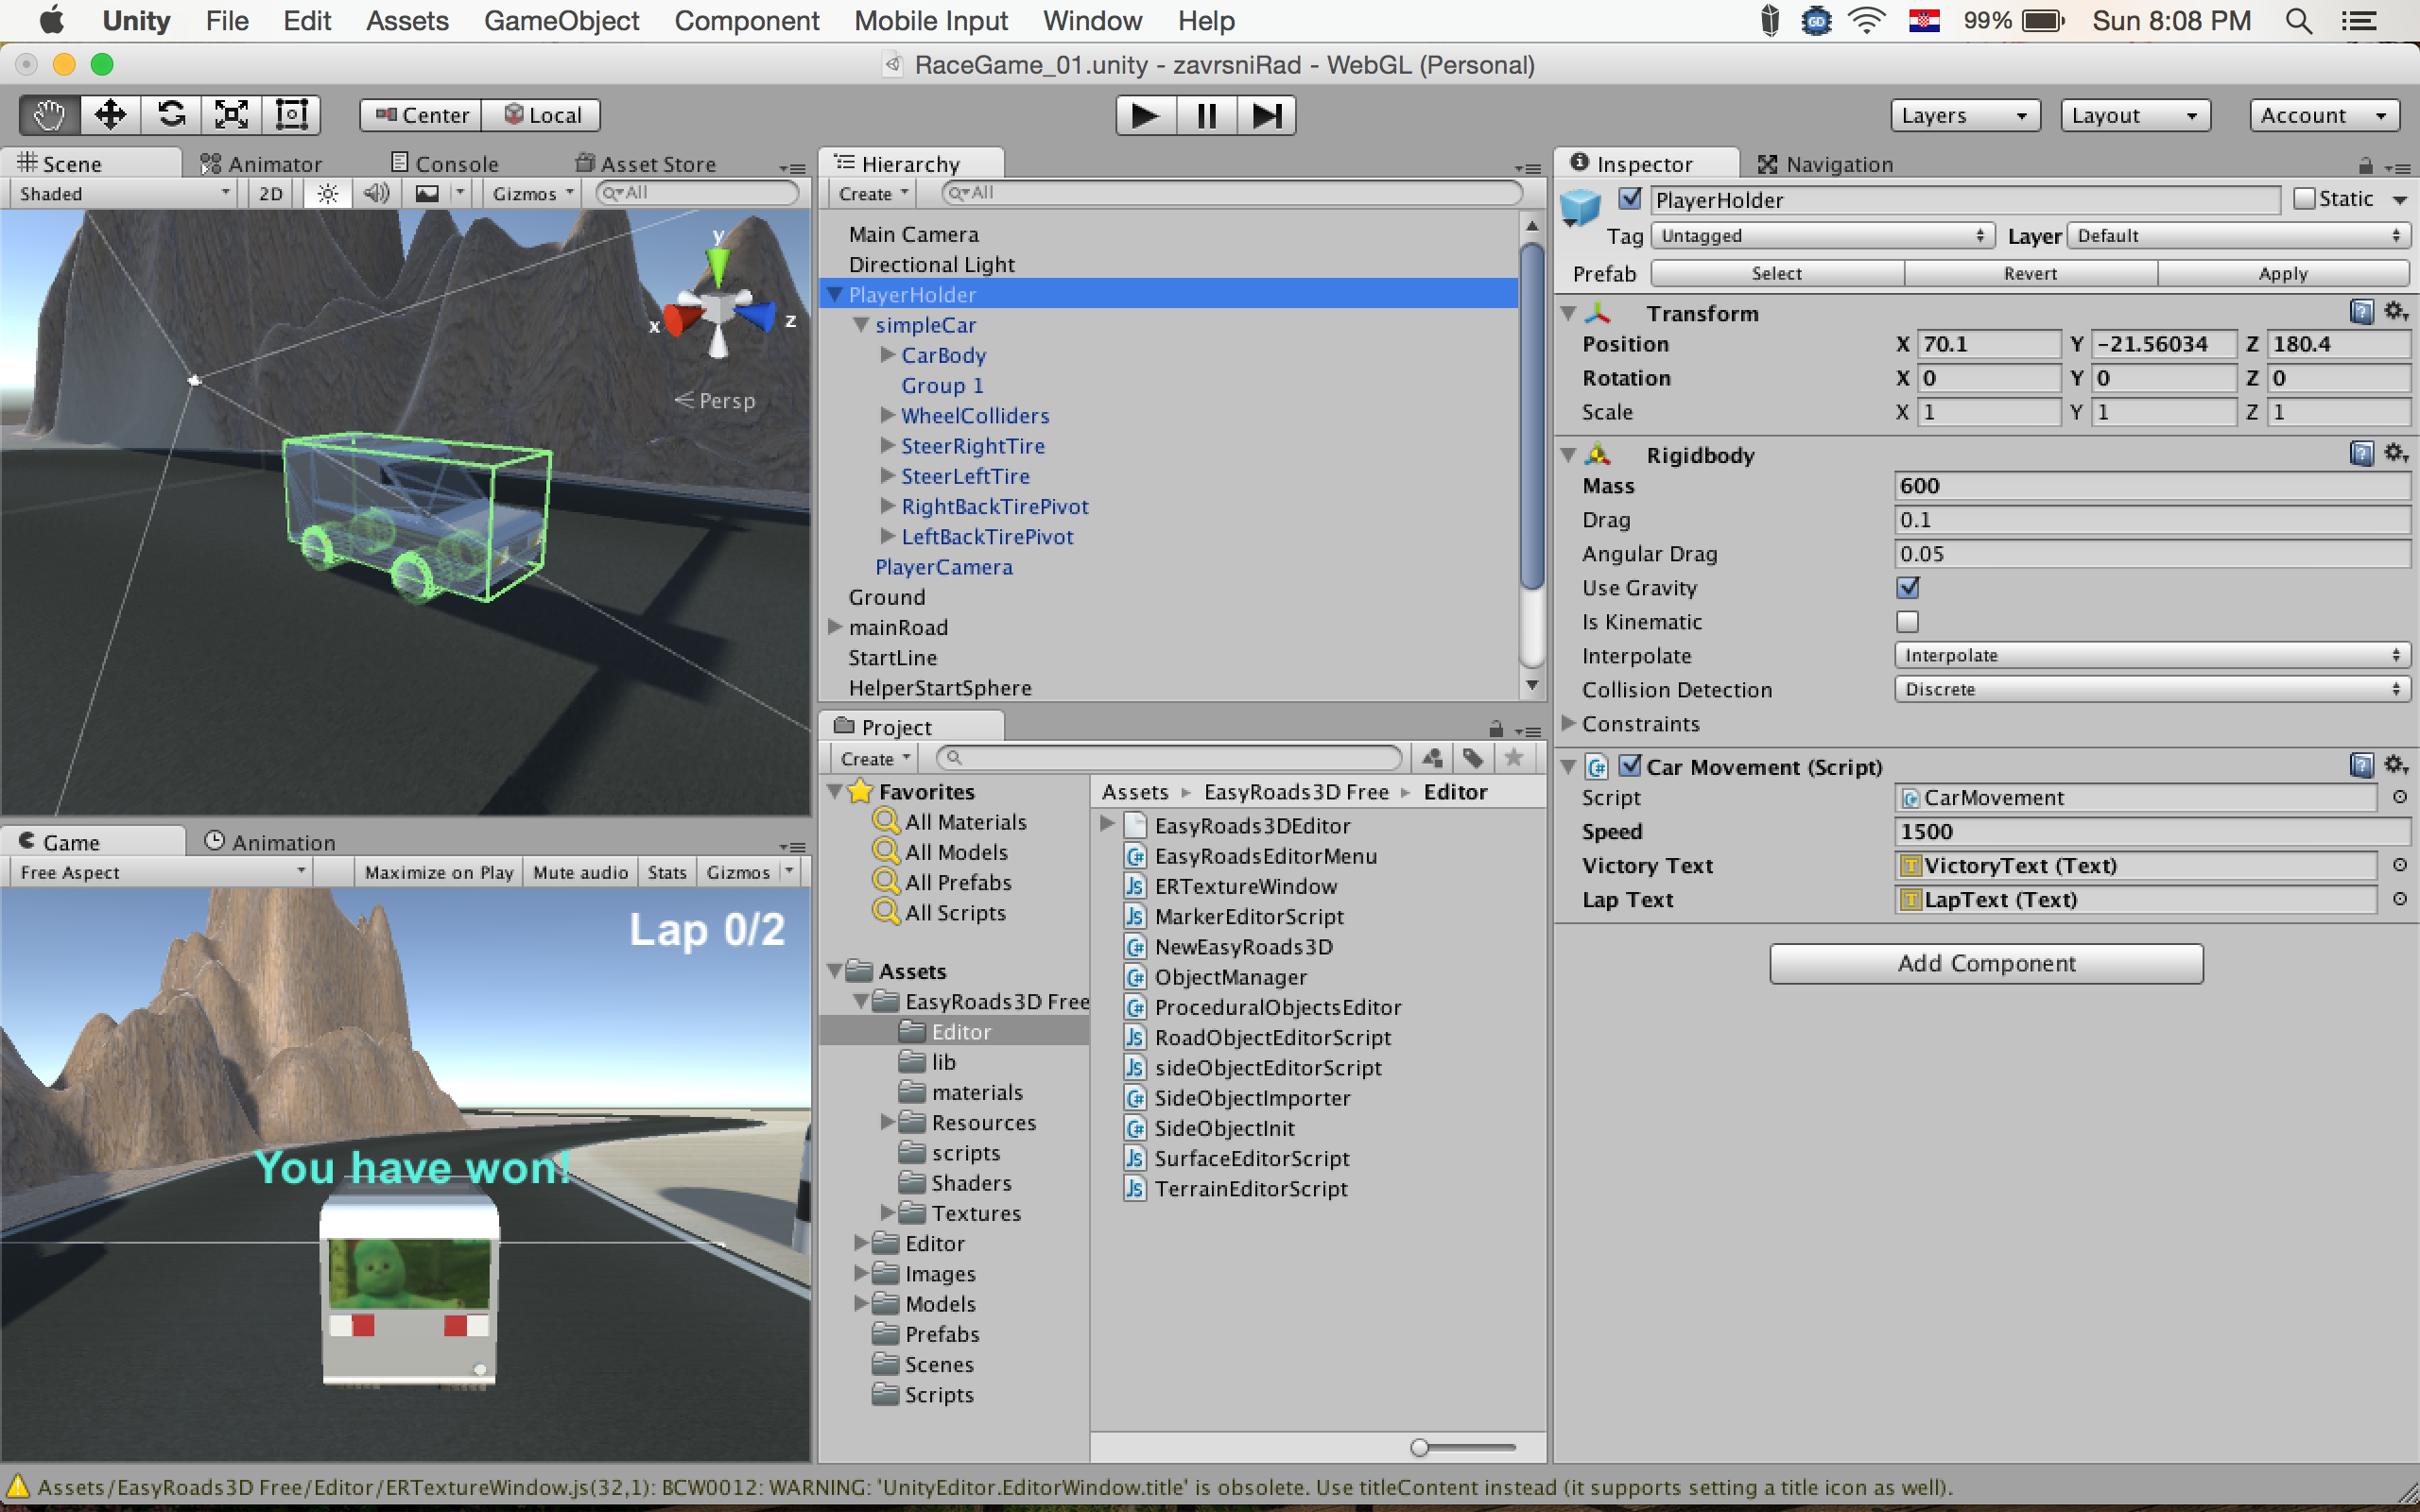
\includegraphics[width=12.5cm, height=10cm]{igrajuci_objekt.png}
	\centering
	\caption{Igrajući objekt}
	\label{fig:igrajuciobjekt}
\end{figure}
\newpage
Na slici broj \ref{fig:igrajuciobjekt} se može vidjeti primjer unity radne okoline i jedan igrajući objekt koji se zove "PlayerHolder". Ovaj igrajući objekt ima tri komponente, transformaciju, kruto tijelo i skriptu koja se zove "CarMovement". O skriptama i kako one funkcioniraju u sljedećem poglavlju. Dodavanje komponenti se može klikom na dugme "Add Component". Nakon klika na dugme se otvara padajući izbornik za odabir željene komponente. \par
Svaki igrajući objekt pripada jednom sloju (\emph{eng. Layer}) i ima oznaku (\emph{eng. Tag}). Kasnije se pomoću skripti može manipulirati ovim elementima provjerom njihovih slojeva i oznaka. U igri se korisei oznake upravo za provjeravanje, da li je korisnik prošao cestu pravim putem. Na slici broj \ref{fig:markeriPutanje} se mogu vidjeti markeri koji provjeravaju navedeno.

\subsection{Kotači}
Kako je navedeno u prethodnom poglavlju kotači se sastoje od više komponenti. Te komponente su mreža (\emph{eng. Mesh}), transformacija, te mrežni prevoditelj (\emph{eng. Mesh Renderer}) koji dopušta korisniku da vidi konačni element. Ono što se koristi za kretanje modela je kolni sudarač. Mreža se može vidjeti na slici \ref{fig:kotaci} desno, a sudarač na slici \ref{fig:kotaci} lijevo. \par
Isto tako veoma bitna stvar je povećati masu modela, inače će početi nekontrolirano rotirati na sceni, kao da je upalo u crnu rupu. Vrijednost u konačnici definira kojom silom će gravitacija privlačiti model, odnosno definiramo brzinu. Što je masa veća sporiji je igrajući objekt i obrnuto.

\begin{figure}[h]
	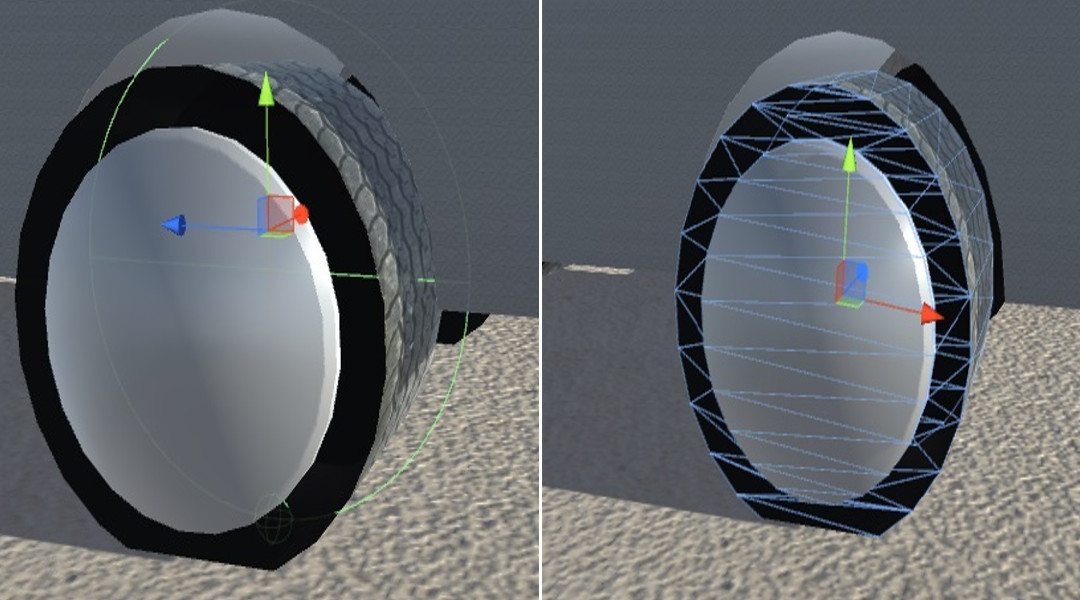
\includegraphics[width=12.5cm, height=7cm]{wheels.jpg}
	\centering
	\caption{Kotači modela}
	\label{fig:kotaci}
\end{figure}

\subsubsection{Rotiranje kotača}
Prilikom vožnje automobila za bolju simulaciju potrebno je okretati i kola. Za isprogramirati ovu naizgled jednostavnu radnju više stvari treba unaprijed biti dobro definirano, inače se stvar komplicira. Ukoliko je igrajući objekt loše definiran i pivoti nisu dobro postavljeni na kotačima, zbog mehanike koju unity koristi objekti rotiraju krivo ili treba koristit naprednije metode koje povećavaju broj linija koda i stvaraju dodatne probleme. 
\newpage
Rotacija kotača bi trebala biti oko njegove osi, te se zato mora postaviti pivot u sredinu kotača. Ovo se obavlja tijekom izrade samog modela, te treba paziti na to prije unosa u unity. Ako se pivot nije centrirao prilikom izrade, onda se treba obavljati popravljanje. Koraci za popravljanje:

\begin{enumerate}
	\item Pronaći objekt (kotač) unutar hijerarhije
	\item Napraviti novi prazni objekt na istoj razini kao i kotač
	\item Kotač ubaciti u prazni objekt
\end{enumerate}
Sada za okretanje kotača se koristi novi prazni objekt jer je njegov pivot centriran. Ovakav pristup je jako učestal zbog dizajnera koji ne paze na pivote unutar svojih modela. Skripta za okretanje kola se može vidjeti u ispisu \ref{okretanjeKola}:
\begin{lstlisting}[caption={Skripta za okretanje kola}, label=okretanjeKola]
for (int i = 0; i < 4; i++) 
			this.tirePivots[i].transform.Rotate(
			    Vector3.forward, 
			    this.speed * move * Time.deltaTime
			);	
\end{lstlisting}

\subsubsection{Problemi u zavojima}
Prilikom vožnje vozila dodavanjem samo kolnih sudarača ne bismo dobili potpunu imitaciju pravog vozila. Jedan od problema koji se javlja je preokretanje u zavojima. Ova pojava je sasvim opravdana i nije nikakva greška programa. Što se ustvari događa? Kada vozilo uđe u zavoj i započme skretanje, na njega djeluje centrifugalna sila, podigne se prednji kotač sa tla i kako ne postoji protusila preokrene se. \par
Za ovaj slučaj postoji više rješenja, a onaj koji se koristi u igrici je sljedeći. Pri skretanju se provjeri koji kotač se podiže od tla i na njega se primjeni sila koja djeluje u smjeru gravitacije. Na ovaj način se smanji utjecaj centrifugalne sile, te samim time teže preokrenuti vozilo.